% to change the appearance of the header, questions, problems or subproblems, see the homework.cls file or
% override the \Problem, \Subproblem, \question or \printtitle commands.

% The hidequestions option hides the questions. Remove it to print the questions in the text.

% CHANGER CE PATH S'IL EST DIFFERENT POUR VOUS
\documentclass[]{../../homework}

\usepackage{booktabs}
\usepackage{graphicx}
\graphicspath{ {./images/} }
\usepackage{mathrsfs}
\usepackage{hyperref}
\usepackage{qrcode}

% Set up your name, the course name and the homework set number.
\homeworksetup{
	username={Thomas Diot, Jim Garnier, Jules Charlier, Pierre Gallois \\ 1E1},
	course={Mathématiques},
	setnumber=1}
\begin{document}% this also prints the header.
	
	\problem*{1}{Logique de Lukasiewicz}
\subproblem Soient $P, Q, R$ trois assertions.
\question Commutativité du "et" :

\begin{tabular}{|c|c|c|c|}
	\hline
	$P$ & $Q$ & $P \land Q$ & $Q \land P$ \\
	\hline
	V   & V   & V            & V            \\
	V   & F   & F            & F            \\
	V   & I   & I            & I            \\
	F   & V   & F            & F            \\
	F   & F   & F            & F            \\
	F   & I   & F            & F            \\
	I   & V   & I            & I            \\
	I   & F   & F            & F            \\
	I   & I   & I            & I            \\
	\hline
\end{tabular}

On observe bien que les colonnes $P \land Q$ et $Q \land P$ sont identiques, donc ces deux assertions sont équivalentes.

\question Associativité du "et" :

\begin{tabular}{|c|c|c|c|c|c|c|}
	\hline
	$P$ & $Q$ & $R$ & $P \land Q$ & $Q \land R$ & $(P \land Q) \land R$ & $P \land (Q \land R)$ \\
	\hline
	V   & V   & V   & V            & V            & V                       & V                       \\
	V   & V   & F   & V            & F            & F                       & F                       \\
	V   & V   & I   & V            & I            & I                       & I                       \\
	V   & F   & V   & F            & F            & F                       & F                       \\
	V   & F   & F   & F            & F            & F                       & F                       \\
	V   & F   & I   & F            & F            & F                       & F                       \\
	V   & I   & V   & I            & I            & I                       & I                       \\
	V   & I   & F   & I            & F            & F                       & F                       \\
	V   & I   & I   & I            & I            & I                       & I                       \\
	F   & V   & V   & F            & V            & F                       & F                       \\
	F   & V   & F   & F            & F            & F                       & F                       \\
	F   & V   & I   & F            & I            & F                       & F                       \\
	F   & F   & V   & F            & F            & F                       & F                       \\
	F   & F   & F   & F            & F            & F                       & F                       \\
	F   & F   & I   & F            & F            & F                       & F                       \\
	F   & I   & V   & F            & I            & F                       & F                       \\
	F   & I   & F   & F            & F            & F                       & F                       \\
	F   & I   & I   & F            & I            & F                       & F                       \\
	I   & V   & V   & I            & V            & I                       & I                       \\
	I   & V   & F   & I            & F            & F                       & F                       \\
	I   & V   & I   & I            & I            & I                       & I                       \\
	I   & F   & V   & F            & F            & F                       & F                       \\
	I   & F   & F   & F            & F            & F                       & F                       \\
	I   & F   & I   & F            & F            & F                       & F                       \\
	I   & I   & V   & I            & I            & I                       & I                       \\
	I   & I   & F   & I            & F            & F                       & F                       \\
	I   & I   & I   & I            & I            & I                       & I                       \\
	\hline
\end{tabular}

On observe bien que les colonnes $(P \land Q) \land R$ et $P \land (Q \land R)$ sont identiques, donc ces deux assertions sont équivalentes.

\question Lois de Morgan :

\begin{tabular}{|c|c|c|c|c|c|c|}
	\hline
	$P$ & $Q$ & $P \vee Q$ & $\lnot P$ & $\lnot Q$ & $\lnot (P \vee Q)$ & $(\lnot P) \land (\lnot Q)$ \\
	\hline
	V   & V   & V          & F         & F         & F                  & F                            \\
	V   & F   & V          & F         & V         & F                  & F                            \\
	V   & I   & V          & F         & I         & F                  & F                            \\
	F   & V   & V          & V         & F         & F                  & F                            \\
	F   & F   & F          & V         & V         & V                  & V                            \\
	F   & I   & I          & V         & I         & I                  & I                            \\
	I   & V   & V          & I         & F         & F                  & F                            \\
	I   & F   & I          & I         & V         & I                  & I                            \\
	I   & I   & I          & I         & I         & I                  & I                            \\
	\hline
\end{tabular}

Les deux dernières colonnes sont identiques, donc $\lnot (P \vee Q) \iff (\lnot P) \land (\lnot Q)$.

\begin{tabular}{|c|c|c|c|c|c|c|}
	\hline
	$P$ & $Q$ & $P \land Q$ & $\lnot P$ & $\lnot Q$ & $\lnot (P \land Q)$ & $(\lnot P) \vee (\lnot Q)$ \\
	\hline
	V   & V   & V            & F         & F         & F                    & F                          \\
	V   & F   & F            & F         & V         & V                    & V                          \\
	V   & I   & I            & F         & I         & I                    & I                          \\
	F   & V   & F            & V         & F         & V                    & V                          \\
	F   & F   & F            & V         & V         & V                    & V                          \\
	F   & I   & F            & V         & I         & V                    & V                          \\
	I   & V   & I            & I         & F         & I                    & I                          \\
	I   & F   & F            & I         & V         & V                    & V                          \\
	I   & I   & I            & I         & I         & I                    & I                          \\
	\hline
\end{tabular}

Les deux dernières colonnes sont identiques, donc $\lnot (P \land Q) \iff (\lnot P) \lor (\lnot Q)$.
On a bien montré que les lois de Morgan restent vérifiées dans $\mathcal{L}_{3}$.

\question On a : \begin{equation*}
	\begin{split}
		P \lor Q &\iff \neg(\neg P \land \neg Q) \\
		&\iff \neg(\neg Q \land \neg P) \\
		&\iff Q \lor P
	\end{split}
\end{equation*}
On a ensuite : \begin{equation*}
	\begin{split}
		(P \lor Q) \lor R &\iff \neg(\neg(P \lor Q) \land \neg R) \\
		&\iff \neg((\neg P \land \neg Q) \land \neg R) \\
		&\iff \neg(\neg P \land (\neg Q \land \neg R)) \\
		&\iff P \lor (Q \lor R)
	\end{split}
\end{equation*}
L'associativité et la commutativité sont donc aussi vérifiées pour la disjonction.

\subproblem Soient $P, Q, R$ trois assertions.
\question\begin{tabular}{|c|c|c|c|c|}
	\hline
	$P$ & $Q$ & $\lnot P$ & $P \Rightarrow Q$ & $(\lnot P) \vee Q$ \\
	\hline
	V   & V   & F         & V                 & V                  \\
	V   & F   & F         & F                 & F                  \\
	V   & I   & F         & I                 & I                  \\
	F   & V   & V         & V                 & V                  \\
	F   & F   & V         & V                 & V                  \\
	F   & I   & V         & V                 & V                  \\
	I   & V   & I         & V                 & V                  \\
	I   & F   & I         & I                 & I                  \\
	I   & I   & I         & V                 & I                  \\
	\hline
\end{tabular}

Les deux dernières colonnes ne sont pas identiques, donc les assertions $(P \Rightarrow Q)$ et $((\lnot P) \vee Q)$ ne sont pas équivalentes dans $\mathcal{L}_{3}$.

\question\begin{tabular}{|c|c|c|c|c|c|}
	\hline
	$P$ & $Q$ & $\lnot P$ & $\lnot Q$ & $P \Rightarrow Q$ & $(\lnot Q) \Rightarrow (\lnot P)$ \\
	\hline
	V   & V   & F         & F         & V                 & V                                 \\
	V   & F   & F         & V         & F                 & F                                 \\
	V   & I   & F         & I         & I                 & I                                 \\
	F   & V   & V         & F         & V                 & V                                 \\
	F   & F   & V         & V         & V                 & V                                 \\
	F   & I   & V         & I         & V                 & V                                 \\
	I   & V   & I         & F         & V                 & V                                 \\
	I   & F   & I         & V         & I                 & I                                 \\
	I   & I   & I         & I         & V                 & V                                 \\
	\hline
\end{tabular}

Les deux dernières colonnes sont identiques, donc on a $(P \Rightarrow Q) \iff ((\lnot Q) \Rightarrow (\lnot P))$. La méthode de démonstration par contraposition est donc toujours valable dans $\mathcal{L}_{3}$.

\question \begin{tabular}{|c|c|c|c|c|c|c|}
	\hline
	$P$ & $Q$ & $R$ & $P \Rightarrow Q$ & $Q \Rightarrow R$ & $(P \Rightarrow Q) \land (Q \Rightarrow R)$ & $P \Rightarrow R$ \\
	\hline
	V   & V   & V   & V                 & V                 & V                                            & V                 \\
	V   & V   & F   & V                 & F                 & F                                            & F                 \\
	V   & V   & I   & V                 & I                 & I                                            & I                 \\
	V   & F   & V   & F                 & V                 & F                                            & V                 \\
	V   & F   & F   & F                 & V                 & F                                            & F                 \\
	V   & F   & I   & F                 & V                 & F                                            & I                 \\
	V   & I   & V   & I                 & V                 & I                                            & V                 \\
	V   & I   & F   & I                 & I                 & I                                            & F                 \\
	V   & I   & I   & I                 & V                 & I                                            & I                 \\
	F   & V   & V   & V                 & V                 & V                                            & V                 \\
	F   & V   & F   & V                 & F                 & F                                            & V                 \\
	F   & V   & I   & V                 & I                 & I                                            & V                 \\
	F   & F   & V   & V                 & V                 & V                                            & V                 \\
	F   & F   & F   & V                 & V                 & V                                            & V                 \\
	F   & F   & I   & V                 & V                 & V                                            & V                 \\
	F   & I   & V   & V                 & V                 & V                                            & V                 \\
	F   & I   & F   & V                 & I                 & I                                            & V                 \\
	F   & I   & I   & V                 & V                 & V                                            & V                 \\
	I   & V   & V   & V                 & V                 & V                                            & V                 \\
	I   & V   & F   & V                 & F                 & F                                            & I                 \\
	I   & V   & I   & V                 & I                 & I                                            & V                 \\
	I   & F   & V   & I                 & V                 & I                                            & V                 \\
	I   & F   & F   & I                 & V                 & I                                            & I                 \\
	I   & F   & I   & I                 & V                 & I                                            & V                 \\
	I   & I   & V   & V                 & V                 & V                                            & V                 \\
	I   & I   & F   & V                 & I                 & I                                            & I                 \\
	I   & I   & I   & V                 & V                 & V                                            & V                 \\
	\hline
\end{tabular}

\subproblem Soient $P, Q$ deux assertions.
\question \begin{tabular}{|c|c|c|c|}
	\hline
	$P$ & $Q$ & $\lnot P$ & $P \vee (\lnot P)$ \\
	\hline
	V   & V   & F         & V                  \\
	V   & F   & F         & V                  \\
	V   & I   & F         & V                  \\
	F   & V   & V         & V                  \\
	F   & F   & V         & V                  \\
	F   & I   & V         & V                  \\
	I   & V   & I         & I                  \\
	I   & F   & I         & I                  \\
	I   & I   & I         & I                  \\
	\hline
\end{tabular}

On observe trois cas où l'assertion $P \vee (\lnot P)$ a la valeur de vérité "I". Ce n'est donc pas une tautologie dans $\mathcal{L}_{3}$.

\question \begin{tabular}{|c|c|c|c|c|}
	\hline
	$P$ & $Q$ & $P \Rightarrow Q$ & $P \land (P \Rightarrow Q)$ & $(P \land (P \Rightarrow Q)) \Rightarrow Q$ \\
	\hline
	V   & V   & V                 & V                            & V                                            \\
	V   & F   & F                 & F                            & V                                            \\
	V   & I   & I                 & I                            & V                                            \\
	F   & V   & V                 & F                            & V                                            \\
	F   & F   & V                 & F                            & V                                            \\
	F   & I   & V                 & F                            & V                                            \\
	I   & V   & V                 & I                            & V                                            \\
	I   & F   & I                 & I                            & I                                            \\
	I   & I   & V                 & I                            & V                                            \\
	\hline
\end{tabular}

On observe un cas où la valeur de vérité de $(P \land (P \Rightarrow Q)) \Rightarrow Q$ est "I". Le principe d'inférence ne vaut donc plus dans $\mathcal{L}_{3}$.

\question \begin{tabular}{|c|c|c|c|c|c|c|}
	\hline
	$P$ & $Q$ & $P \Rightarrow Q$ & $\lnot P$ & $(\lnot P) \Rightarrow Q$ & $(P \Rightarrow Q) \land ((\lnot P) \Rightarrow Q)$ & $((P \Rightarrow Q) \wedge ((\lnot P) \Rightarrow Q)) \Rightarrow Q$ \\
	\hline
	V   & V   & V                 & F         & V                         & V                                                    & V                                                                    \\
	V   & F   & F                 & F         & V                         & F                                                    & V                                                                    \\
	V   & I   & I                 & F         & V                         & I                                                    & V                                                                    \\
	F   & V   & V                 & V         & V                         & V                                                    & V                                                                    \\
	F   & F   & V                 & V         & F                         & F                                                    & V                                                                    \\
	F   & I   & V                 & V         & I                         & I                                                    & V                                                                    \\
	I   & V   & V                 & I         & V                         & V                                                    & V                                                                    \\
	I   & F   & I                 & I         & I                         & I                                                    & I                                                                    \\
	I   & I   & V                 & I         & V                         & V                                                    & I                                                                    \\
	\hline
\end{tabular}

Dans deux cas l'assertion $((P \Rightarrow Q) \wedge ((\lnot P) \Rightarrow Q)) \Rightarrow Q$ prend la valeur de vérité "I". Ce n'est donc pas une tautologie dans $\mathcal{L}_{3}$.
\\
\\
	
	
	
	
	\problem*{2}{Triangles magiques}
	\partie{A}{Questions Préliminaires}
		On cherche à encadrer la somme $S = a + b+ c$ quand $a,b$ et $c$ sont des entiers distincts entre $1$ et $9$. Sans perte de généralité, supposons que $a < b < c$ : c'est possible, car les trois entiers sont distincts et peuvent être intervertis si l'ordre n'est pas respecté.
	\par \underline{Borne inférieure pour S :} On remarque que $6 \leq S$, en prenant $S = 1 + 2 + 3$. Prouvons que cette valeur est minimale. Pour minimiser $S$, on doit choisir $a = 1$, sinon $S' = (a-1) + b + c$ serait plus petite. Par le même raisonnement, on doit choisir $b=2$ et $c=3$, car $a,b,c$ sont distincts. Donc $6$ est bien la plus petite valeur que peut prendre $S$.
	\par \underline{Borne supérieure pour S :} On raisonne de la même manière. Afin de maximiser $S$, on doit choisir $c=9$, sinon $S' = a+b+(c+1) > S$. Comme $b<c$, il s'ensuit qu'on a nécessairement $b=8$ et enfin $a=7$. Ainsi la valeur maximale que peut prendre $S$ est $S=7+8+9 = 24$.
	
	\par \underline{Conclusion :} $6 \leq S \leq 24$.
	
	\partie{B}{Les triangles magiques}
	\subproblem{}
	
	Le triangle suivant est $20$-magique :
	
	\begin{center}
	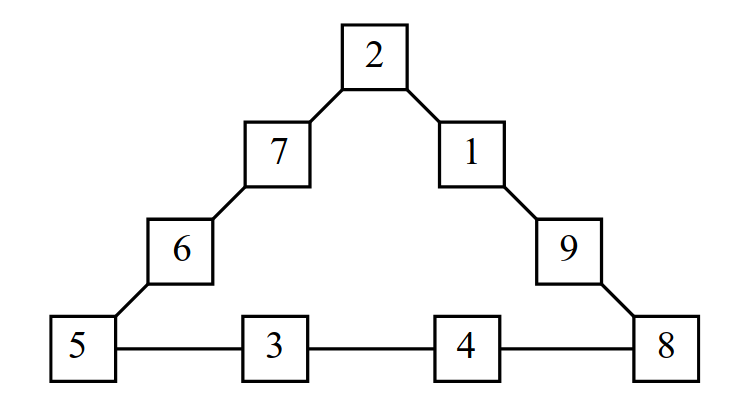
\includegraphics[scale=0.3]{20-magique}
	\end{center}
	
	\subproblem{}
	\question
	Comme $S = n_1 + n_2 + n_3 + n_4 = n_4+n_5+n_6+n_7 = n_7 + n_8 + n_9 + n_1$, on somme les trois valeurs pour trouver :
	\begin{equation*}
		3S = (n_1 + n_2 + n_3 + n_4 +n_5+n_6+n_7 + n_8 + n_9) + (n_1 + n_4 + n_7)
	\end{equation*}
	Comme les nombres $n_1,\dots,n_9$ sont les nombres de $1$ à $9$ dans le désordre, leur somme vaut $1 + 2 + \dots + 9=45$. De plus, $n_1$, $n_4$ et $n_7$ sont les nombres aux sommets du triangle. Donc $n_1 + n_4 + n_7 = T$. On trouve donc enfin :
	\begin{equation}
		3S = 45 + T
	\end{equation}
	
	\question
	Avec la partie A, on sait que $T$, étant la somme de trois entiers entre $1$ et $9$, a l'encadrement $6 \leq T \leq 24$. Donc $\frac {6+45} {3} \leq S \leq \frac {24+45} 3$, ce qui donne $17 \leq S \leq 23$.
	\question 
	Les couples $(S,T)$ possibles sont :

\begin{table}[!h]
	\centering
	\begin{tabular}{|l|l|}
		\hline
		\multicolumn{1}{|c|}{S}  & T  \\ \hline
		\multicolumn{1}{|c|}{17} & 6  \\ \hline
		\multicolumn{1}{|c|}{18} & 9  \\ \hline
		\multicolumn{1}{|c|}{19} & 12 \\ \hline
		20                       & 15 \\ \hline
		21                       & 18 \\ \hline
		22                       & 21 \\ \hline
		23                       & 24 \\ \hline
	\end{tabular}
\end{table}
	Où les valeurs de $T$ sont calculées avec $(1)$ en fonction de celles de $S$

	\subproblem
	Comme le triangle recherché est $17$-magique, alors $T = 6$. Donc $T = 1 + 2 + 3$ et les nombres sur les sommets doivent être $1$, $2$ et $3$. On trouve donc le triangle $17$-magique suivant :
	
	\begin{center}
	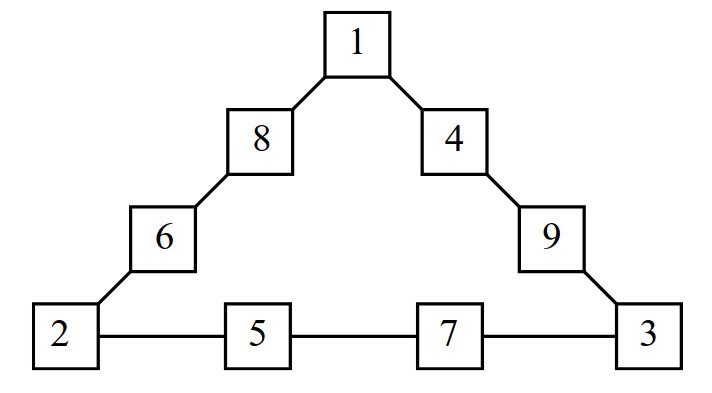
\includegraphics[scale=0.3]{17-magique}
	\end{center}
	\subproblem
	On prouve d'abord le lemme suivant, qui sera utile dans le reste du sujet.
	
	\begin{lemma}
		Si un triangle est $S$-magique et que le nombre $n=S-T$ est compris entre 1 et 9, alors $n$ est sur l'un des sommets du triangle.
	\end{lemma}
	\begin{proof}
		On se place dans les conditions de l'énoncé. Prouvons par l'absurde que $n$ est sur le triangle, en supposant qu'il se trouve sur l'un des côtés mais pas sur les sommets. Notons $a,b$ les extrémités du côté sur lequel se trouve $n$ et $x$ le dernier nombre de ce côté.
			
		Par hypothèse, $a+b+x+n =S$. Donc $a+b+x = T$ car $n=S-T$. Comme $a$ et $b$ sont fixés, $x$ doit être égal au nombre qui se trouve sur le 3e sommet du triangle. C'est une contradition, car tous les nombres d'un triangle $S$-magique sont distincts. Donc $n$ est sur un sommet du triangle.
	\end{proof}
	
	Ainsi, si un triangle $18$-magique existe, alors $9$ doit se trouver sur l'un des sommets du triangle. Mais comme $T = 9$, la somme des deux autres nombres sur les sommets du triangle doit valoir $0$, ce qui est impossible. Donc il n'existe pas de triangle $18$-magique.
	
	\subproblem
	\question Par le lemme ci-dessus, comme $19-12 = S-T = 7$, $7$ doit se trouver sur l'un des sommets du triangle.
	\question Le triangle suivant est $19$-magique :

	\begin{center}
	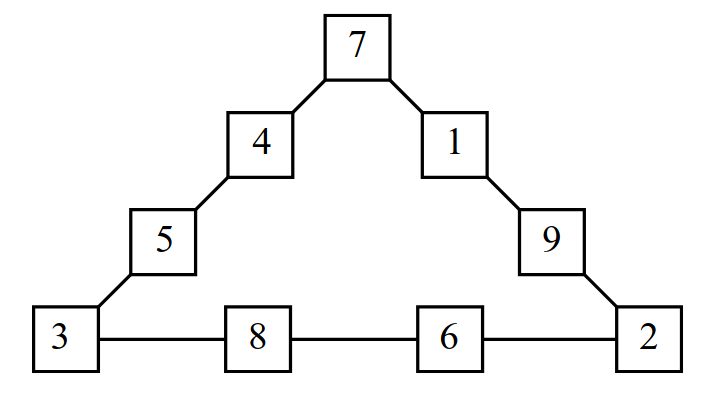
\includegraphics[scale=0.3]{19-magique}
	\end{center}
	
	\subproblem
	Remplaçons chaque $n_i, i\in [\![1,9]\!]$ par $n'_i = 10-n_i$. Cette transformation est valide : les entiers $n'_i$ sont toujours compris entre $1$ et $9$, et restent distincts. Si la somme des nombres d'un côté vaut $S$, la somme des $n_i'$ de ce côté est $40-S$. Donc, si un triangle est $S$-magique, alors il existe un triangle $(40-S)$-magique. \\

	\subproblem
	On a prouvé qu'il existe des triangles $20$, $17$ et $19$-magiques. D'après $6)$, il existe donc des triangles $23$ et $21$-magiques. On a aussi prouvé qu'il n'existe pas de triangle $18$-magique. Reste enfin le cas $S = 22$.
	
	Par la contraposée de $6)$, s'il n'existe pas de triangle $40-22=18$-magique, alors il n'existe pas de triangle $22$-magique. Comme il n'existe pas de triangle $18$-magique, il n'existe pas de triangle $22$-magique.
"
	On résume donc les valeurs de $S$ pour lesquelles il existe un triangle $S$-magique dans le tableau suivant :
	\begin{table}[!h]
		\centering
		\begin{tabular}{|l|l|l|}
			\hline
			\multicolumn{1}{|c|}{S}            & T                & Existe \\ \hline
			\multicolumn{1}{|c|}{\textless 17} & \textless 6      & Non    \\ \hline
			\multicolumn{1}{|c|}{17}           & 6                & Oui    \\ \hline
			\multicolumn{1}{|c|}{18}           & 9                & Non    \\ \hline
			\multicolumn{1}{|c|}{19}           & 12               & Oui    \\ \hline
			20                                 & 15               & Oui    \\ \hline
			21                                 & 18               & Oui    \\ \hline
			22                                 & 21               & Non    \\ \hline
			23                                 & 24               & Oui    \\ \hline
			\textgreater 23                    & \textgreater{}24 & Non    \\ \hline
		\end{tabular}
	\end{table}

\section*{Sources}
\begin{itemize}
	\item Le site de l'APMEP pour les images de triangles complétés, afin de ne pas avoir à les faire avec \LaTeX
	\item \url{https\detokenize{:}//www.overleaf.com/latex/templates/template-for-rapid-homework-typesetting/rycccpxphchn} pour le template du devoir
\end{itemize}
Les tables de vérité de ce devoir maison ont été générées grâce à un programme de notre création disponible ici. (\url{https\detokenize{:}//github.com/DArtagnant/automatic-latex-truth-table-builder})
Celui est capable de générer les tables de vérité en \LaTeX de toute assertion dans $\mathscr{L}_2$ ou $\mathscr{L}_3$.
\begin{center}
	\protect\qrcode[height=1in]{https\detokenize{:}//github.com/DArtagnant/automatic-latex-truth-table-builder}
\end{center}

\end{document}